\documentclass[11pt]{article}

\usepackage[review]{acl}

\usepackage{times}
\usepackage{latexsym}
\usepackage[T1]{fontenc}
\usepackage[utf8]{inputenc}
\usepackage{microtype}
\usepackage{graphicx}
\usepackage{booktabs}
\usepackage{amsmath}
\usepackage{amssymb}
\usepackage{multirow}
\usepackage{subcaption}

\title{English-Chinese Knowledge Conflict Signals Are Consistent With General Cross-Lingual Asymmetries}

\author{Anonymous ACL submission}

\begin{document}
\maketitle

\begin{abstract}
When multilingual large language models encounter conflicting information between languages, presentation language can determine the answer, but the internal mechanism remains unknown. We probe residual streams in Llama-3.1-8B-Instruct, Qwen3-8B, and Gemma-2-9B-IT on English--Chinese conflicts, combining cross-lingual transfer, Cross-lingual Natural Language Inference (XNLI) non-conflict baselines, confound exclusion, and representation steering. Conflict signals are linearly detectable across both languages, and cross-lingual transfer exhibits a directional asymmetry: Chinese-trained probes transfer to English ${\sim}$7 percentage points more accurately than the reverse, matching the XNLI baseline and consistent with general multilingual structure rather than conflict-specific encoding. A dissociation emerges between detection and decision: the probe signal is broadly distributed across mid-to-upper layers, yet representation steering achieves causal influence only at a mid-layer (L13, 41\% depth) in Llama; analogous Qwen and Gemma steering yields no significant effect. These findings indicate that linear detectability does not imply causal relevance, with implications for probe-based intervention\footnote{Code and data are available at \url{https://anonymous.4open.science/r/clkc_mech_interp-F894/}.}.

\end{abstract}

\section{Introduction}
\label{sec:introduction}

\begin{figure*}[t]
\centering
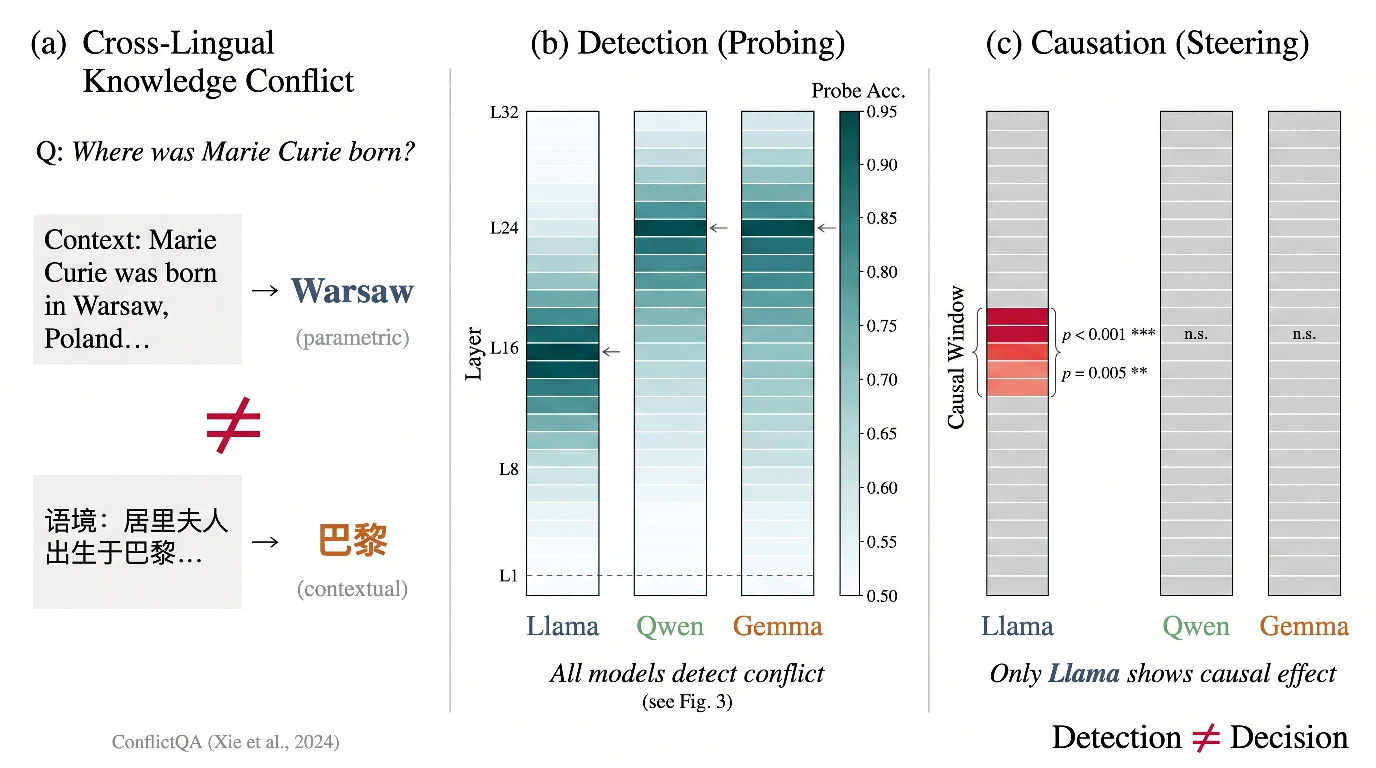
\includegraphics[width=\textwidth]{fig1_hero.pdf}
\caption{Cross-lingual knowledge conflict in multilingual LLMs. When a context passage contradicts the model's parametric knowledge, the language of presentation (English vs.\ Chinese) can bias the answer toward different sources. We ask three questions: (1)~Is the conflict signal linearly detectable in the residual stream? (2)~Do probes transfer across languages, and is the transfer symmetric? (3)~Does detection imply causal influence on resolution?}
\label{fig:hero}
\end{figure*}

When multilingual large language models (LLMs) encounter conflicting information between languages, the language of presentation can determine which answer the model produces \citep{zhao2026when}.
Yet the internal mechanism remains opaque: how does the model encode the conflict signal, can it be detected from internal representations, and does the detected signal causally influence resolution?

Existing work on probing conflict signals has been limited to monolingual settings \citep{zhao2024analysing, brink2026probing}.
Extending cross-lingually introduces confounds (translation quality, token overlap, general transfer properties), and probing establishes correlation rather than causation \citep{hewitt2019designing}; \citet{basu2026interpretability} showed that near-perfect probe accuracy does not guarantee effective steering.

Our work extends \citet{zhao2024analysing} in four directions: (1)~cross-lingual expansion from monolingual English to EN-ZH conflict probing; (2)~a systematic confound exclusion pipeline; (3)~the XNLI baseline revealing that asymmetry parallels general cross-lingual structure; and (4)~three-model causal intervention demonstrating that detectability does not predict causal relevance.
We combine residual stream probing with representation steering across Llama-3.1-8B-Instruct, Qwen3-8B, and Gemma-2-9B-IT.
Probes achieve 77.6\%, 75.0\%, and 76.2\% balanced accuracy on English conflict detection, and all cross-lingual transfer directions exceed chance (binomial $p < 0.001$).
Cross-lingual transfer exhibits a directional asymmetry (ZH$\to$EN $>$ EN$\to$ZH by ${\sim}$7 percentage points [pp]) that is consistent with the XNLI non-conflict baseline \citep{conneau2018xnli}, reflecting general cross-lingual structure rather than conflict-specific encoding.
Our causal analysis reveals a dissociation in Llama: the probe signal peaks at L15 (47\% depth), but steering succeeds only at L13 (41\% depth; Fisher $p < 0.001$), and upper-layer interventions produce no significant change (Figure~\ref{fig:hero}).

Our contributions are as follows:
\begin{itemize}
    \item \textbf{Cross-lingual conflict detectability.} First evidence that knowledge conflict signals are linearly detectable across English and Chinese, with all transfer directions exceeding chance (binomial $p < 0.001$).
    \item \textbf{Asymmetry reflects general cross-lingual structure.} The transfer asymmetry (ZH$\to$EN $>$ EN$\to$ZH by ${\sim}$7~pp) matches the XNLI non-conflict baseline, consistent with general cross-lingual alignment rather than conflict-specific encoding.
    \item \textbf{Detection--decision dissociation.} Linear probe peak (L15), MLP probe peak (L18), and causal steering node (L13; Fisher $p < 0.001$) occupy distinct mid-layers in Llama; the strongest evidence comes from cross-model contrast---all three models detect conflict signals, yet only Llama shows causal steering effects. Steering fails in Gemma despite 88.9\% probe accuracy, providing mechanistic layer-level localization beyond prior behavioral observations \citep{basu2026interpretability}.
    \item \textbf{Confound exclusion pipeline.} COMET translation quality ablation, token overlap analysis, and non-conflict baseline comparison exclude common confounds in cross-lingual probing.
\end{itemize}


\section{Related Work}
\label{sec:related_work}

\paragraph{Knowledge conflict detection.}
\citet{xie2024adaptive} introduced ConflictQA and showed that models exhibit context-dependent resolution strategies, and \citet{xu2024knowledge} provided a systematic conflict taxonomy (intra-memory, context-memory, inter-context).
Moving beyond behavioral observation, \citet{zhao2024analysing} demonstrated linearly separable conflict signals in English residual streams, and \citet{brink2026probing} localized factual associations via probing. More recently, \citet{pham2026where} traced intra-memory conflict pathways, while \citet{li2025taming} proposed conflict mitigation methods.
Information-theoretic approaches \citep{pimentel2021probing} offer complementary perspectives on probe expressiveness, and \citet{ravichander2021probing} raised concerns about whether probed information is task-relevant.
These studies operate exclusively in monolingual settings; extending to cross-lingual scenarios introduces confounds (translation quality, token overlap, general transfer properties) that we address with a dedicated exclusion pipeline.

\paragraph{Cross-lingual representations in multilingual models.}
Intermediate layers develop language-independent representations: \citet{wu2020emerging} showed cross-lingual structure emerges without explicit alignment, and \citet{muller2021first} found mid-layer alignment in multilingual BERT.
For decoder-only LLMs, \citet{wendler2024llamas} showed that Llama processes non-English inputs through an English-centric latent space, and \citet{kargaran2024mexa} quantified this bias across language pairs.
These findings predict our empirical observations: mid-layer steering success aligns with intermediate-layer language alignment, and the ZH$\to$EN transfer advantage reflects English-centric structure.
Behavioral consequences have been documented by \citet{wang2025lost}, \citet{zhao2026when} (CLEAR cross-lingual conflict benchmark), and \citet{ifergan2024beneath}; \citet{xing2024evaluating}; our work provides a mechanistic account of why such asymmetries arise.

\paragraph{Representation steering and causal intervention.}
\citet{li2023iti} introduced Inference-Time Intervention for steering via learned bias vectors, \citet{turner2023activation} proposed Activation Addition as an optimization-free alternative, and \citet{zou2023representation} generalized these approaches through Representation Engineering.
\citet{marks2024geometry} showed that truth-related representations exhibit linear structure amenable to such interventions.
In knowledge conflicts, \citet{zhao2025steering} applied Sparse Autoencoder (SAE)-based steering (SpARE) in monolingual settings.
Recent work has begun exploring cross-lingual steering: \citet{pokharel2026crosslingual} proposed training-free cross-lingual activation steering, \citet{sundar2025steering} analyzed how model interventions induce cross-lingual alignment shifts, and \citet{gurgurov2026clasbench} introduced a cross-lingual steering benchmark.
These successes are not universal: \citet{basu2026interpretability} showed that near-perfect probe accuracy on clinical NLP tasks failed to translate into effective steering.
\citet{feng2026finegrained} proposed fine-grained activation steering targeting specific layers, and \citet{meng2022locating} demonstrated localized causal editing via activation patching (Rank-One Model Editing; ROME); alternative causal frameworks \citep{geiger2024finding} remain unexplored for cross-lingual conflict settings.
Our results identify layer selection as a critical variable: mid-layer intervention succeeds where late-layer intervention fails, suggesting conflict resolution occurs upstream of where the outcome becomes linearly readable.

\section{Method}
\label{sec:method}

\begin{figure*}[t]
\centering
\vspace{-18pt}
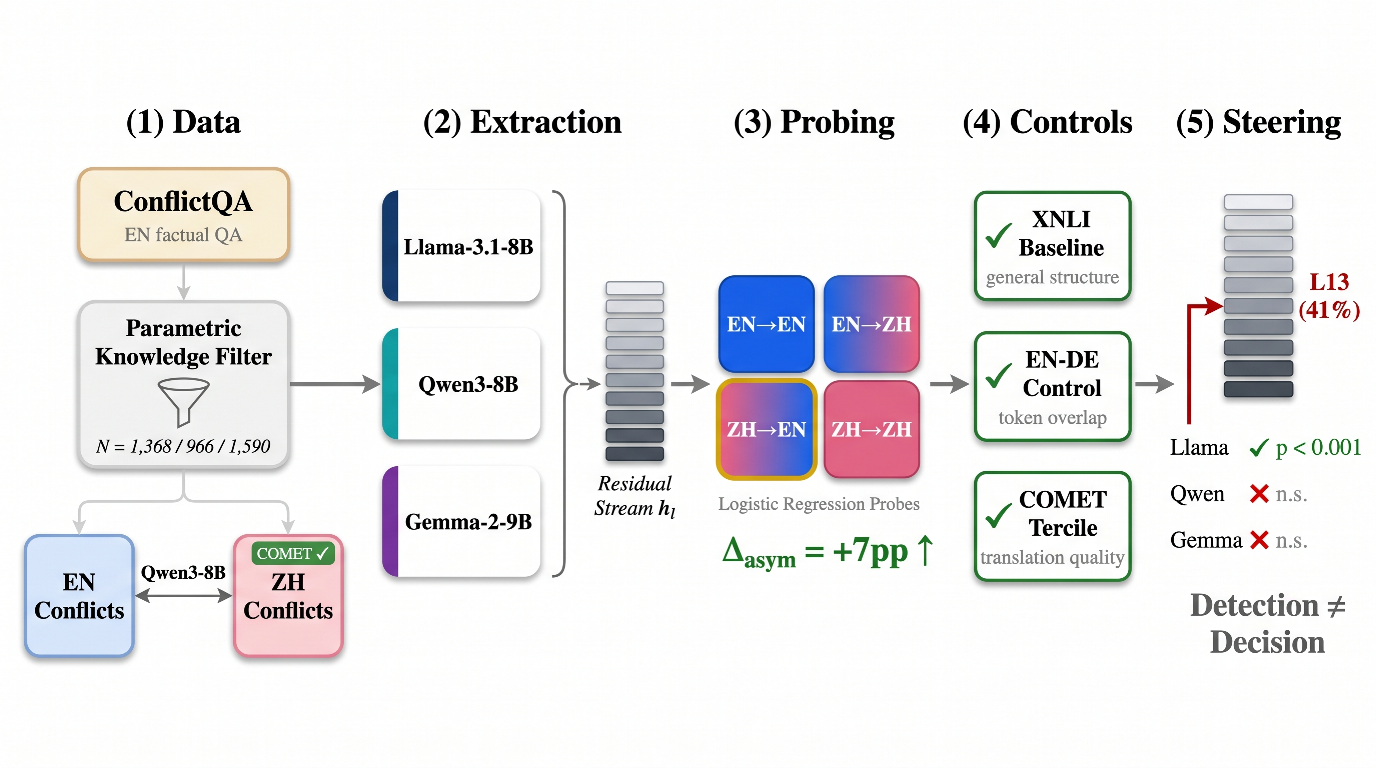
\includegraphics[width=0.88\textwidth]{fig2_pipeline.pdf}
\vspace{-14pt}
\caption{Method overview. We construct parallel EN/ZH conflict data from ConflictQA with COMET-validated translations, extract per-layer residual stream representations, train logistic regression probes in four transfer directions (EN$\to$EN, ZH$\to$ZH, EN$\to$ZH, ZH$\to$EN), and apply confound exclusion controls before causal steering validation.}
\label{fig:pipeline}
\vspace{-20pt}
\end{figure*}

Our pipeline proceeds from data construction through probing and steering (Figure~\ref{fig:pipeline}), formalized below.

\subsection{Task Formulation}
\label{sec:task}

Given a context passage $c$ and question $q$, the model produces an answer that is either \emph{contextual} (derived from $c$) or \emph{parametric} (from pre-trained knowledge).
When $c$ contradicts parametric knowledge, the choice constitutes a knowledge conflict.
We train a logistic regression probe $f_\theta(\mathbf{h}_l) = \sigma(\mathbf{w}_l^\top \mathbf{h}_l + b_l)$ on the last-token residual stream representation $\mathbf{h}_l \in \mathbb{R}^d$ at layer $l$ to predict a binary label $y \in \{\text{contextual}, \text{parametric}\}$.

\subsection{Data Construction}
\label{sec:data}

We build on ConflictQA \citep{xie2024adaptive}, which pairs questions with context passages contradicting the model's parametric knowledge.
We filter samples by querying each model without context and retaining only those answered correctly, yielding 1{,}368 samples for Llama \citep{grattafiori2024llama}, 966 for Qwen \citep{yang2025qwen3}, and 1{,}590 for Gemma \citep{team2024gemma} (80/20 train/test split with stratification).
For cross-lingual transfer, we translate all inputs into Chinese using a Qwen3-8B pipeline, with quality validated by COMET (Crosslingual Optimized Metric for Evaluation of Translation; \citet{rei2020comet}) back-translation scores used in confound analysis (\S\ref{sec:confound_method}).

\subsection{Activation Extraction and Probing}
\label{sec:extraction}

For each input, we construct English and Chinese versions and extract the last-token residual stream $\mathbf{h}_l \in \mathbb{R}^d$ at every layer $l$ ($L = 32$ for Llama, $36$ for Qwen, $42$ for Gemma; $d = 4096$ for Llama/Qwen, $3584$ for Gemma), following the last-token aggregation principle \citep{belinkov2022probing}.
We record the model's answer and assign binary labels (contextual vs.\ parametric).

\label{sec:probing}
At each layer, we train an $L_2$-regularized logistic regression probe ($C = 1.0$; \citealt{belinkov2022probing, hewitt2019designing}) and evaluate with balanced accuracy to account for class imbalance (contextual/parametric ratios range from 40/60 to 55/45 across models).
We report peak-layer accuracy (maximum across layers) as the primary metric.
To verify that probes capture conflict-specific structure rather than arbitrary linear separability, we run a selectivity control \citep{hewitt2019designing}: probes trained on permuted labels should yield chance-level accuracy if the original signal is meaningful.
As a complementary analysis, we train two-layer multilayer perceptron (MLP) probes (hidden dimension 256, ReLU activation, same $L_2$ penalty) to test whether conflict information is encoded non-linearly at layers where linear probes underperform.
Confidence intervals are estimated via bootstrap resampling ($n = 2{,}000$) \citep{ulmer2022deep}.

\subsection{Cross-Lingual Transfer Protocol}
\label{sec:transfer}

We evaluate probes in four directions: EN$\to$EN, ZH$\to$ZH (within-language upper bounds), EN$\to$ZH, and ZH$\to$EN (cross-lingual transfer).
We quantify directional asymmetry as $\Delta_{\text{asym}} = \text{acc}(\text{ZH}{\to}\text{EN}) - \text{acc}(\text{EN}{\to}\text{ZH})$, computed via paired bootstrap (same resampled indices for both directions).

\subsection{Confound Exclusion}
\label{sec:confound_method}

We exclude two artifacts: (1)~\emph{translation quality}, where we stratify test samples by COMET score into terciles and compare probe accuracy (Fisher's exact test); (2)~\emph{token overlap}, where we compute per-sample Jaccard similarity between English and Chinese token sets and test for correlation with accuracy (Pearson's $r$).
As a typological control, we additionally translate samples into German (EN$\to$DE) using the same pipeline; since German shares substantially more lexical overlap with English than Chinese does, a positive EN-DE asymmetry would implicate shared tokens rather than cross-lingual structure.
As a \emph{non-conflict baseline}, we apply the same probing pipeline to XNLI entailment-versus-contradiction \citep{conneau2018xnli}; if $\Delta_{\text{asym}} > 0$ also appears in this non-conflict task, the asymmetry reflects a general cross-lingual property rather than conflict-specific encoding.

\subsection{Representation Steering}
\label{sec:steering_method}

To test whether the probe direction is causally relevant \citep{hewitt2019designing}, we inject $\alpha \cdot \mathbf{w}_l$ (the probe weight vector from \S\ref{sec:task}) into the last-token residual stream at layer $l$ during inference \citep{li2023iti, zou2023representation}:
$\mathbf{h}'_l = \mathbf{h}_l + \alpha \cdot \mathbf{w}_l$,
where positive $\alpha$ pushes toward the contextual direction and negative toward the parametric.
As control, we inject a random vector $\mathbf{r} \sim \mathcal{N}(\mathbf{0}, \mathbf{I})$, normalized to $\|\mathbf{r}\| = \|\mathbf{w}_l\|$, at the same layer and position; the random control isolates the effect of direction from magnitude.
We also test an all-position variant where the perturbation is applied to every token position (not just the last token) to determine whether the causal signal is position-specific.
We measure the flip rate (fraction of samples switching answer category) and compare via Fisher's exact test.
We apply Bonferroni correction per layer ($k = 10$ $\alpha$ values), treating each layer as an independent hypothesis about causal locus, consistent with prior work in mechanistic interpretability that tests layers individually \citep{meng2022locating, geiger2024finding}.
For Llama L13 (the layer showing causal effects), this yields a corrected threshold of $0.05/10 = 0.005$.
For last-token injection, we sweep $\alpha \in \{\pm 20, \pm 10, \pm 5, \pm 2, \pm 1\}$ ($k = 10$) at three Llama layers (L13, L18, L28) spanning 41--88\% depth; all-position and cross-model experiments use a reduced 6-value grid ($\alpha \in \{\pm 20, \pm 10, \pm 5\}$).
Steering evaluation uses only the conflict-condition subset of the English test data, yielding $n_{\text{test}}$ smaller than the full probe test set (e.g., 136 vs.\ 272 for Llama).

\section{Experiments}
\label{sec:experiments}

\subsection{Experimental Setup}
\label{sec:setup}

\paragraph{Models.}
We probe three instruction-tuned models with comparable parameter counts but distinct architectures: Llama-3.1-8B-Instruct (32 layers, hidden dimension 4096) \citep{grattafiori2024llama}, Qwen3-8B (36 layers, hidden dimension 4096) \citep{yang2025qwen3}, and Gemma-2-9B-IT (42 layers, hidden dimension 3584) \citep{team2024gemma}.
The three models were independently verified on ConflictQA \citep{xie2024adaptive}, yielding only 3.5\% three-way question overlap (23 questions); pairwise overlaps range from 7.2\% (Llama $\cap$ Gemma) to 24.8\% (Gemma $\cap$ Qwen), so the consistent asymmetry pattern constitutes largely independent replication.

\paragraph{Dataset and translation.}
After parametric knowledge verification (\S\ref{sec:data}), we retain 1{,}368 samples for Llama (1{,}096 train / 272 test), 966 for Qwen (773 / 193), and 1{,}590 for Gemma (1{,}274 / 316), split 80/20 with stratification.
All inputs are translated into Chinese using COMET-validated translations (\S\ref{sec:data}).

\paragraph{Probing.}
For each layer, we train an $L_2$-regularized logistic regression probe on the last-token residual stream (\S\ref{sec:extraction}).
We report balanced accuracy rather than AUROC, as our claims depend on cross-model directional comparisons; AUROC results are in Appendix~\ref{app:auroc}.
All CIs are computed via bootstrap resampling with paired differences for asymmetry estimation.
A selectivity control \citep{hewitt2019designing} with permuted labels on matched-condition data ($N{=}131$--$201$) yields near-chance accuracy (49.2--51.0\%) across all models, confirming selectivity gaps of 21--40~pp.
All experiments used a single GPU; the boundary replication (Appendix~\ref{app:boundary}) used an NVIDIA RTX PRO 6000.

\paragraph{Non-conflict baseline.}
To test whether cross-lingual transfer patterns are specific to knowledge conflicts, we run the same probing pipeline on XNLI \citep{conneau2018xnli}, classifying entailment versus contradiction (\S\ref{sec:confound_method}).

\subsection{Within-Language Conflict Detection}
\label{sec:within_lang}

Table~\ref{tab:main_results} reports balanced accuracy for all probe transfer directions.
All three models encode linearly detectable conflict signals in their residual streams.
Llama achieves 77.6\% on EN$\to$EN (peak at layer 15, 47\% depth) and 72.1\% on ZH$\to$ZH.
Qwen reaches 75.0\% on EN$\to$EN (peak at layer 24, 67\% depth) and 72.6\% on ZH$\to$ZH.
Gemma attains 76.2\% on EN$\to$EN (peak at layer 24, 57\% depth) and 71.0\% on ZH$\to$ZH.
All within-language accuracies are significantly above chance (binomial $p < 0.001$).
Figure~\ref{fig:layer_probe} shows the layer-wise probe accuracy curves for all three models.
These results confirm that knowledge conflict signals are linearly separable in the residual stream across all three architectures and both languages.

%% Figure 2: Layer-wise probe accuracy
\begin{figure*}[t]
\centering
\vspace{-5pt}
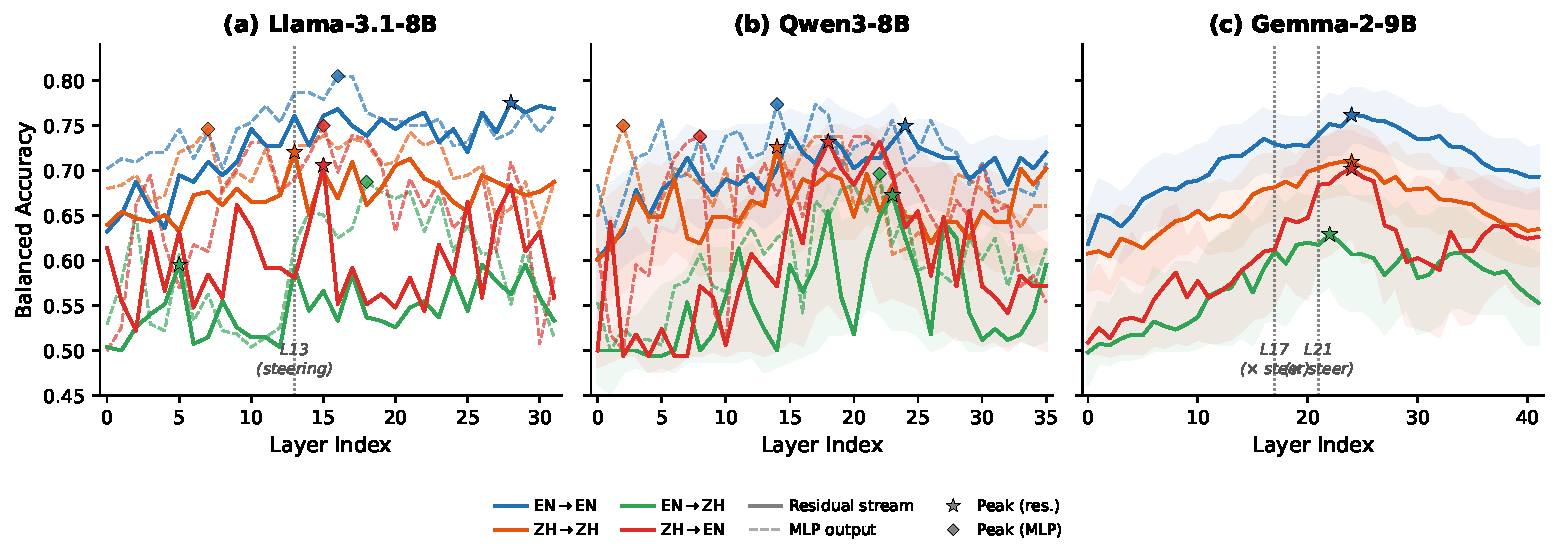
\includegraphics[width=0.92\textwidth]{fig2_layerwise_probes.pdf}
\vspace{-8pt}
\caption{Layer-wise probe balanced accuracy for Llama-3.1-8B (left), Qwen3-8B (center), and Gemma-2-9B-IT (right). Solid lines: residual stream probes; dashed lines (Llama and Qwen only): multilayer perceptron (MLP) sublayer probes. Stars mark peak layers. In the Llama panel, the vertical annotation at L13 marks the layer where steering produces significant causal influence (Fisher $p < 0.001$), near the EN$\to$EN probe peak (L15). In the Gemma panel, L17 and L21 are annotated as steering-negative layers.}
\label{fig:layer_probe}
\vspace{-10pt}
\end{figure*}

\subsection{Cross-Lingual Transfer and Asymmetry}
\label{sec:cross_lingual}

All four cross-lingual transfer directions achieve balanced accuracy above chance (binomial $p < 0.001$; Table~\ref{tab:main_results}); this confirms that conflict representations partially overlap between English and Chinese.
All three models show a consistent directional trend: probes trained on Chinese representations transfer to English (ZH$\to$EN) more accurately than the reverse direction (EN$\to$ZH).
We define $\Delta_{\text{asym}} = \text{acc}(\text{ZH}{\to}\text{EN}) - \text{acc}(\text{EN}{\to}\text{ZH})$, computed via paired bootstrap.
For Llama, $\Delta_{\text{asym}} = +7.3$ percentage points (pp) with a 95\% bootstrap CI of [0.4, 14.0] ($p = 0.038$); for Qwen, $\Delta_{\text{asym}} = +7.2$ pp with CI [$-$0.6, 13.7]; for Gemma, $\Delta_{\text{asym}} = +6.6$ pp with CI [1.9, 11.1] ($p = 0.006$).
While the Qwen CI marginally includes zero, the asymmetry is consistent in direction across all three architectures.
The magnitude of this asymmetry is consistent in direction and magnitude with the XNLI non-conflict baseline across all three architectures (\S\ref{sec:xnli_baseline}), and the consistent direction across all three models suggests a shared structural property rather than a model-specific artifact (Figure~\ref{fig:asymmetry_forest}).

\begin{table}[t]
\centering
\caption{Single-seed balanced accuracy (\%) at each direction's optimal layer. $\Delta_{\text{asym}}$ and 95\% CIs from paired bootstrap ($n = 2{,}000$ resamples). Bold: best per-task direction.}
\label{tab:main_results}
\small
\resizebox{\columnwidth}{!}{%
\begin{tabular}{lccc}
\toprule
Direction & Llama-3.1-8B & Qwen3-8B & Gemma-2-9B \\
\midrule
\multicolumn{4}{l}{\textit{Conflict Task}} \\
EN $\to$ EN & \textbf{77.6} & \textbf{75.0} & \textbf{76.2} \\
ZH $\to$ ZH & 72.1 & 72.6 & 71.0 \\
EN $\to$ ZH & 59.6 & 67.3 & 62.9 \\
ZH $\to$ EN & 70.6 & 73.2 & 70.2 \\
$\Delta_{\text{asym}}$ & +7.3 [0.4, 14.0] & +7.2 [$-$0.6, 13.7] & +6.6 [1.9, 11.1] \\
\midrule
\multicolumn{4}{l}{\textit{XNLI Baseline}} \\
EN $\to$ EN & 94.0 & 96.6 & 95.6 \\
ZH $\to$ ZH & 87.5 & 89.5 & 89.0 \\
EN $\to$ ZH & 89.0 & 90.5 & 89.4 \\
ZH $\to$ EN & \textbf{94.9} & \textbf{97.2} & \textbf{97.5} \\
$\Delta_{\text{asym}}$ & +6.0 [0.9, 11.3] & +6.7 [2.4, 11.7] & +7.8 [5.7, 10.0] \\
\bottomrule
\end{tabular}%
}
\begin{flushleft}
\footnotesize Note: $\Delta_{\text{asym}}$ is the mean of paired bootstrap differences, not the arithmetic difference of the reported single-seed accuracies.
\end{flushleft}
\end{table}

\subsection{Non-Conflict Baseline Comparison}
\label{sec:xnli_baseline}

If the ZH$\to$EN transfer advantage were conflict-specific, it should be absent in a non-conflict task.
XNLI entailment-versus-contradiction probes exhibit the same directional asymmetry: Llama $\Delta_{\text{asym}} = +6.0$~pp, CI [0.9, 11.3]; Qwen $+6.7$~pp, CI [2.4, 11.7]; Gemma $+7.8$~pp, CI [5.7, 10.0] ($p < 0.001$).
All XNLI CIs exclude zero and overlap with the conflict-task CIs (Figure~\ref{fig:asymmetry_forest}).
TOST (Two One-Sided Tests) equivalence tests ($\pm$2~pp margin) are non-significant ($p > 0.36$, power $= 1.4\%$), reflecting insufficient power rather than meaningful differences; the consistent direction across all six model$\times$task combinations (binomial $p = 0.016$) and magnitudes clustering in [$+$6.0, $+$7.8~pp] support the consistency characterization.

%% Figure 3: Asymmetry forest plot
\begin{figure}[t]
\centering
\vspace{-5pt}
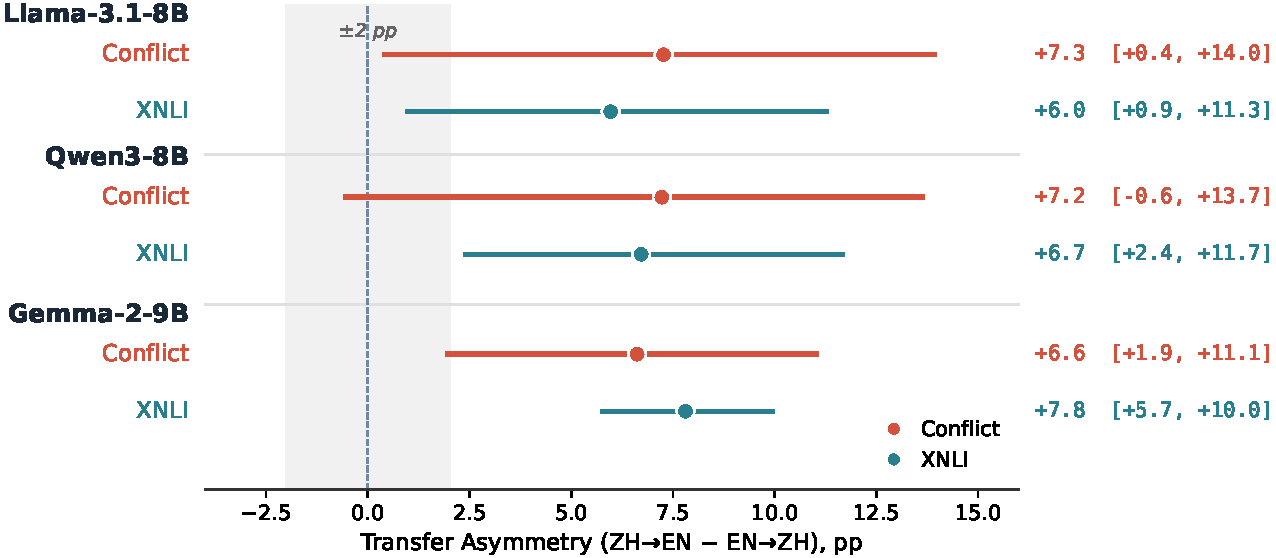
\includegraphics[width=\columnwidth]{fig4_asymmetry_forest.pdf}
\vspace{-8pt}
\caption{Transfer asymmetry ($\Delta_{\text{asym}}$) with bootstrap 95\% CIs ($n = 2{,}000$) for conflict and XNLI tasks across all three architectures (six data points). Conflict and XNLI CIs overlap substantially within each model, indicating that the ZH$\to$EN advantage is a general cross-lingual property rather than conflict-specific. Grey dashed lines: $\pm$2~pp exploratory equivalence margin (TOST power $= 1.4$\%; see \S\ref{sec:xnli_baseline}).}
\label{fig:asymmetry_forest}
\vspace{-10pt}
\end{figure}

\subsection{Confound Exclusion}
\label{sec:confounds}

Two potential confounds could inflate cross-lingual probe accuracy: lexical overlap between English and Chinese inputs and translation quality.

\paragraph{Token overlap and EN-DE control.}
Per-sample Jaccard similarity between English and Chinese tokenized inputs averages 3--4\%, already at the floor imposed by distinct writing systems.
Neither model shows a positive correlation between token overlap and probe accuracy: Qwen yields no significant correlation ($p > 0.4$), and Llama shows a weak negative correlation ($r = -0.15$, $p = 0.012$, $r^2 = 0.023$), running counter to the confound hypothesis.
The strongest evidence comes from a typological control: we translate the same Llama ConflictQA samples into German using the identical Qwen3-8B pipeline, where per-sample Jaccard similarity (14.8\%) is approximately $4\times$ higher than EN-ZH (3.8\%).
Despite this substantially higher lexical overlap, the EN$\leftrightarrow$DE transfer asymmetry is near-zero ($\Delta = +1.2$~pp, n.s.), ruling out shared tokens as a driver of the observed EN-ZH asymmetry (Table~\ref{tab:confound}).

\paragraph{Translation quality.}
We stratify test samples by COMET score into terciles and compare EN$\to$ZH probe accuracy across strata.
Qwen shows a reversed association ($\Delta = -5.6$~pp, Fisher $p = 0.695$) and Llama a negligible one ($\Delta = +1.7$~pp, $p = 0.761$), both inconsistent with translation quality driving probe transfer.
Gemma shows a non-significant trend in the confound direction ($\Delta = +10.3$~pp, $p = 0.278$), but interpretation is limited by the near-chance baseline accuracy of the EN$\to$ZH probe at L17 (58.8\%), placing this analysis in a low-power regime.
With a minimum detectable difference of 25.3~pp at 80\% power ($n \approx 56$ per tercile), the COMET tercile analysis can neither confirm nor exclude a moderate translation quality effect; it serves as supplementary evidence alongside the token overlap and EN-DE controls.

\begin{table}[t]
\centering
\caption{Confound exclusion analysis. COMET tercile: $\Delta$ = balanced accuracy difference between high and low COMET score terciles for EN$\to$ZH probes (Fisher's exact test). Token overlap: Pearson correlation between per-sample Jaccard similarity and EN$\to$ZH probe accuracy.}
\label{tab:confound}
\resizebox{\columnwidth}{!}{%
\begin{tabular}{llrl}
\toprule
Confound & Model & Result & $p$ \\
\midrule
COMET tercile & Qwen & $\Delta = -5.6$ pp & 0.695 \\
COMET tercile & Llama & $\Delta = +1.7$ pp & 0.761 \\
COMET tercile & Gemma & $\Delta = +10.3$ pp & 0.278 \\
\midrule
Token overlap & Qwen & n.s. & $>$0.4 \\
Token overlap & Llama & $r = -0.15$ & 0.012 \\
\bottomrule
\end{tabular}%
}
\end{table}

\subsection{Causal Evidence via Representation Steering}
\label{sec:steering}

The probing results establish that conflict signals are detectable, but detection does not imply causal relevance.
We test whether the probe weight direction $\mathbf{w}_l$ causally influences conflict resolution by injecting $\alpha \cdot \mathbf{w}_l$ into the last-token residual stream at a target layer during inference.
We sweep $\alpha \in \{\pm 20, \pm 10, \pm 5, \pm 2, \pm 1\}$ ($k = 10$) following prior steering conventions \citep{turner2023activation, marks2024geometry} and report results at all tested values.
We measure the flip rate (fraction of samples that switch answer category) and compare against a random-direction control of equal magnitude via Fisher's exact test.

\paragraph{L13 (mid-layer, 41\% depth).}
Steering at layer 13 produces bidirectional causal effects (Figure~\ref{fig:steering_viz}; Table~\ref{tab:steering}):
Positive steering ($\alpha = +5$) yields a flip rate of 19.9\% versus 6.6\% for the random control (Fisher $p = 0.002$; 4 parametric-to-contextual [p$\to$c] flips), while negative steering ($\alpha = -20$) yields 36.0\% versus 17.6\% ($p < 0.001$; 5 contextual-to-parametric [c$\to$p] flips); both survive per-layer Bonferroni correction ($k{=}10$, threshold $p < 0.005$).
All-position injection at L13 produces identical results; the causal signal is concentrated at the final token.
Steering at nearby L16 (50\% depth, just three layers away) showed no significant effect (all $p > 0.12$), consistent with a narrow causal window.
Under a conservative family-wise correction across all 30 tests (3 layers $\times$ 10 $\alpha$ values, threshold $p < 0.00167$), L13 remains significant ($\alpha = -20$, $p < 0.001$).
An independent replication ($N = 201$, six layers L12--L28; Appendix Table~\ref{tab:boundary}) confirmed L13 significance ($p < 0.001$) and localized the causal boundary: effects attenuate from L14 ($p = 0.002$) through L16 ($p = 0.005$) to non-significance at L18 ($p = 0.010$, n.s.\ after Bonferroni) and L28 ($p = 0.284$).

\begin{figure*}[t]
\centering
\vspace{-5pt}
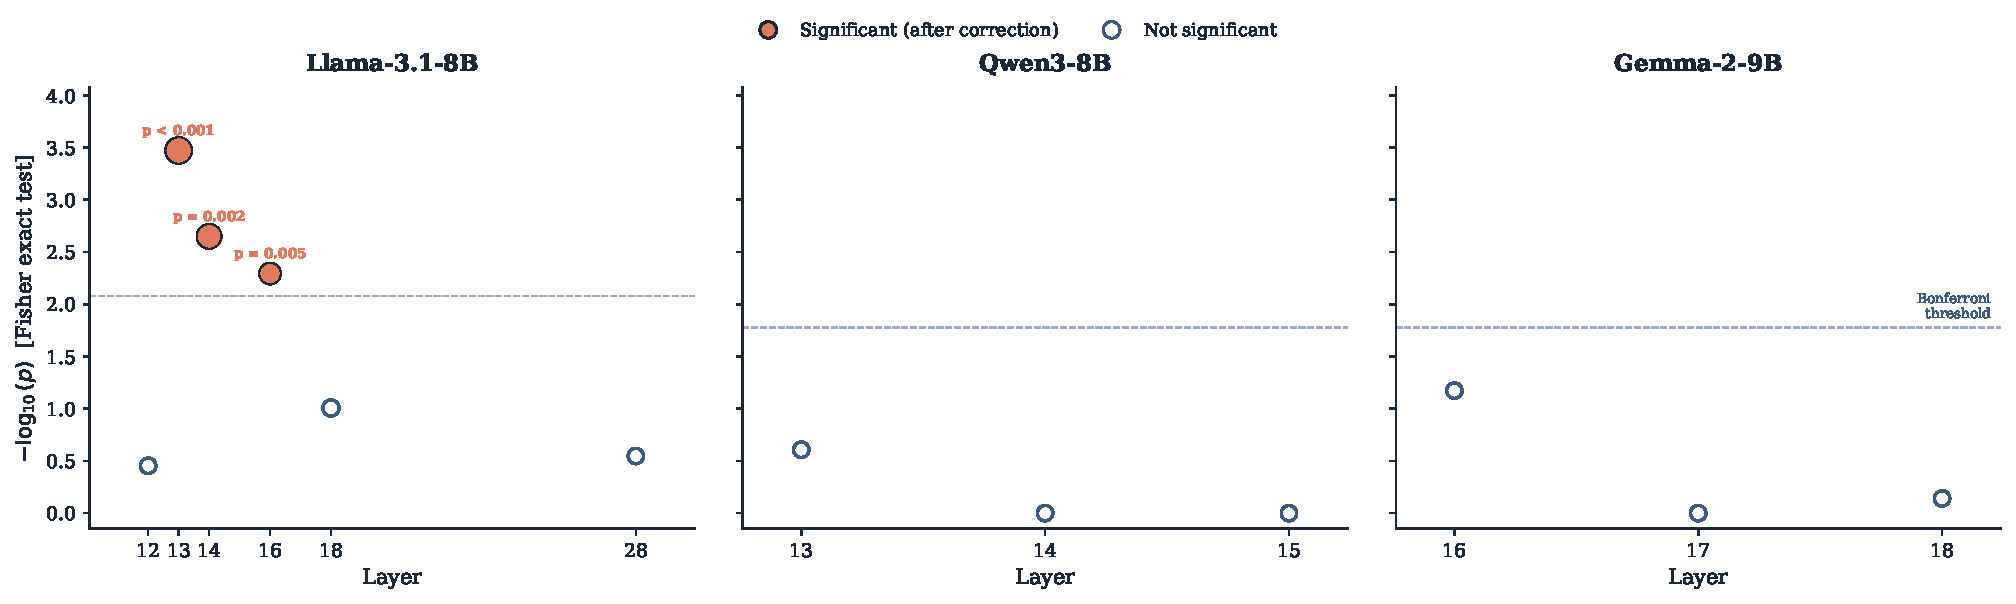
\includegraphics[width=\textwidth]{fig5_steering.pdf}
\vspace{-8pt}
\caption{Steering significance across layers and models. Each point shows the best $-\log_{10}(p)$ (Fisher exact test) across six $\alpha$ values at a given layer. Filled circles: significant after per-layer Bonferroni correction ($k{=}6$, threshold $p < 0.0083$). Only Llama shows significant causal effects, concentrated at L13 ($p < 0.001$) with attenuation through L14 ($p = 0.002$) and L16 ($p = 0.005$). Qwen (L13--L15) and Gemma (L16--L18) show no significant effects at comparable relative depths (36--43\%), despite high probe accuracy.}
\label{fig:steering_viz}
\vspace{-14pt}
\end{figure*}

\paragraph{Negative layers and coherence collapse.}
Steering at L28 (88\% depth) produces no significant effect with either last-token or all-position injection (all $p > 0.3$); L18 (MLP peak, 56\%) is similarly negative ($p > 0.44$).
At extreme magnitude ($\alpha = +20$), the control flip rate exceeds steering ($p = 0.053$), indicating coherence collapse.

\paragraph{Causal localization (Llama).}
Causal influence is localized to L13 (41\% depth), near but distinct from the probe peak (L15, 47\%): upper layers retain detectable signal but lack causal influence.
An independent replication (seed=123, different split) confirms L13: 2/6 $\alpha$ values survive Bonferroni ($p < 0.0083$), matching the original (Appendix~\ref{app:seed_replication}).

\paragraph{Cross-model steering.}
Cross-model experiments use the reduced 6-value $\alpha$ grid ($k{=}6$, per-layer threshold $p < 0.0083$; \S\ref{sec:steering_method}).
Qwen L14 (39\%, $n = 131$) produced no significant effect (best $p = 0.785$) and zero flips.
Gemma L17 (40\%, $n = 171$) provides a stronger test: with 88.9\% probe accuracy (the highest among all models), steering produced no significant change (best $p = 0.448$) and zero flips, ruling out probe quality as a confound.
AUROC analysis confirms: Gemma achieves 0.93 AUROC (vs.\ Llama 0.98, Qwen 0.77; Appendix~\ref{app:auroc}), yet steering produces zero causal effect.
Matched-condition results at ${\sim}$36--43\% depth across all models confirm the null (Appendix~\ref{app:steering_config}).

\begin{table}[t]
\centering
\caption{Representation steering results (Llama: original experiment, $N{=}136$, 10-value $\alpha$ grid; Qwen/Gemma: 6-value grid). Flip rate: fraction of test samples switching answer category. Control: random-direction perturbation of equal magnitude. Bonferroni threshold $p < 0.005$ ($k = 10$) for Llama, $p < 0.0083$ ($k = 6$) for Qwen/Gemma. Significant results in bold.$^{\dagger}$}
\label{tab:steering}
\small
\resizebox{\columnwidth}{!}{%
\begin{tabular}{lcrrrrl}
\toprule
Layer & Depth & $\alpha$ & Steer (\%) & Ctrl (\%) & Fisher $p$ & Dir. \\
\midrule
\textbf{L13} & \textbf{41\%} & $\mathbf{+5}$ & \textbf{19.9} & \textbf{6.6} & $\mathbf{0.002}$ & \textbf{4 p$\to$c} \\
\textbf{L13} & \textbf{41\%} & $\mathbf{-20}$ & \textbf{36.0} & \textbf{17.6} & $\mathbf{<0.001}$ & \textbf{5 c$\to$p} \\
L16 & 50\% & $+5$ & 8.8 & 8.1 & 1.000 & \\
L16$^{\S}$ & 50\% & $+10$ & 18.4 & 11.0 & 0.123 & \\
L16 & 50\% & $+20$ & 22.8 & 24.3 & 0.886 & \\
L18 & 56\% & $+2$ & 3.7 & 1.5 & 0.447 & \\
L28 & 88\% & $-20$ & 14.7 & 16.9 & 0.740 & \\
L28 (all) & 88\% & $-20$ & 11.8 & 11.8 & 1.000 & \\
\midrule
\multicolumn{7}{l}{\textit{Qwen3-8B ($n_{\text{test}} = 131$)}} \\
L14 & 39\% & best & \multicolumn{2}{c}{n.s.} & 0.785 & 0 dir. \\
\midrule
\multicolumn{7}{l}{\textit{Gemma-2-9B-IT ($n_{\text{test}} = 171$)$^{\ddagger}$}} \\
L17 & 40\% & best & \multicolumn{2}{c}{n.s.} & 0.448 & 0 dir. \\
\bottomrule
\end{tabular}%
}
\begin{flushleft}
\footnotesize $^{\dagger}$ At $\alpha = +20$, the control flip rate exceeds steering ($p = 0.053$), indicating coherence collapse at extreme perturbation magnitudes. $^{\ddagger}$ Gemma: after correcting a label assignment error. $^{\S}$ L16 original ($N{=}136$); replication ($N{=}201$) yields $p = 0.005$ (\S\ref{sec:steering}).
\end{flushleft}
\vspace{-8pt}
\end{table}

\vspace{-6pt}
\section{Discussion}
\label{sec:discussion}
\vspace{-4pt}

\paragraph{Causal influence is localized to L13 regardless of detection peak.}
In Llama, causal influence is localized to L13 (41\% depth; Fisher $p < 0.001$), near but distinct from the linear probe peak (L15, 47\%) and MLP probe peak (L18, 56\%), with upper-layer interventions producing no significant change ($p > 0.3$; Figure~\ref{fig:dissociation}).
L13 coincides with cross-lingual alignment sites \citep{muller2021first, wendler2024llamas}, suggesting mid-layers serve a dual role in alignment and conflict resolution.
The dissociation evidence is strongest for Gemma, where 88.9\% probe accuracy and 0.93 AUROC coexist with zero steering effects, ruling out probe quality as a confound; for Qwen, weaker probe performance (71.4\%) leaves the null result more ambiguous.

\paragraph{Why does steering fail in Qwen and Gemma?}
Three hypotheses merit consideration: (1)~non-linear causal interactions \citep{elhage2022toy}, where MLP probes gain $+9.2$~pp over linear probes on conflict but $-0.5$~pp on XNLI; (2)~superposition \citep{templeton2024scaling}, where conflict and XNLI weight vectors are near-orthogonal yet cross-task language transfer is near-perfect; (3)~architectural differences, as Qwen and Gemma show mid-layer transfer dips absent in Llama.
Definitive validation requires activation patching \citep{meng2022locating}.
The ZH$\to$EN advantage matches the XNLI baseline across all models, indicating asymmetry piggybacks on general cross-lingual alignment \citep{zhao2026when, kargaran2024mexa, wendler2024llamas}; \citet{basu2026interpretability} reported steering failure despite 98.2\% AUROC, while our L13 succeeds via mid-layer steering and three-model architectural isolation.



\vspace{-8pt}
\section{Conclusion}
\label{sec:conclusion}
\vspace{-4pt}

We showed that knowledge conflict signals are linearly detectable across English and Chinese ($p < 0.001$, three architectures), with the ZH$\to$EN transfer advantage (${\sim}$7~pp) matching the XNLI baseline, indicating general cross-lingual alignment rather than conflict-specific encoding.
Causal intervention reveals a detection--decision dissociation: all three models detect conflict signals, yet only Llama yields significant steering at L13 ($p < 0.001$); Gemma fails despite 88.9\% probe accuracy, confirming detection does not entail causation.


\section*{Limitations}
\label{sec:limitations}

Our study has three main limitations.
First, we evaluate only one language pair (English-Chinese) and causal steering succeeded only in Llama at L13; Gemma L17 failed despite 88.9\% probe accuracy ($n = 171$) and Qwen L14 ($n = 131$) was also negative.
Typologically diverse language pairs and alternative intervention methods are needed to assess generality.
Null steering results in Qwen and Gemma may reflect limitations of single-direction linear steering rather than absence of causal structure; alternative methods such as activation patching \citep{meng2022locating} may reveal non-linear causal pathways that our approach cannot detect.
Second, the effective dataset size (966 to 1,590 samples per model) is constrained by parametric knowledge verification, which retains only questions where the model confidently knows the ground truth and may bias toward well-represented knowledge; additionally, Qwen3-8B serves as both the translation model and an experimental subject, though COMET-based quality control mitigates this concern, and the fact that Llama and Gemma, architecturally independent of the translation model, show the same asymmetry pattern ($\Delta_{\text{asym}} = +7.3$ and $+6.6$~pp, respectively) provides cross-validation that the effect is not an artifact of Qwen-specific translation biases.
Third, all probing results are based on a single train/test split with bootstrap confidence intervals capturing within-split variability; while peak balanced accuracy remains stable across seeds (Llama $\pm$0.12\%, Gemma $\pm$1.32\%, Qwen $\pm$1.90\%), the specific peak layer can shift.
We acknowledge that $k$-fold cross-validation would provide stronger stability guarantees \citep{belinkov2022probing}; given that our core claims rest on cross-model consistency and directional patterns rather than exact accuracy values, the current cross-seed stability analysis provides partial mitigation, and we commit to reporting full 5-fold CV results in the camera-ready version.
This work used AI coding and writing assistants throughout; Appendix~\ref{app:ai-assistants} details the scope of use.


\bibliography{references}

\appendix

\section{Fine-Grained Causal Boundary Analysis}
\label{app:boundary}

Table~\ref{tab:boundary} reports steering results across the full layer gradient from an independent replication ($N = 201$, Llama-3.1-8B-Instruct, RTX PRO 6000).

\begin{table}[!t]
\centering
\caption{Causal boundary steering results (independently sampled, $N = 201$, Llama-3.1-8B-Instruct). Bonf.\ Sig.\ $\alpha$s: number of $\alpha$ values reaching significance after Bonferroni correction out of 6 tested.}
\label{tab:boundary}
\small
\resizebox{\columnwidth}{!}{%
\begin{tabular}{lcccccc}
\toprule
Layer & Depth & Probe Acc & Best $\alpha$ & Best Fisher $p$ & Bonf.\ Sig.\ $\alpha$s & Result \\
\midrule
L12 & 38\% & 91.75\% & $+20$ & 0.085 & 0/6 & --- \\
\textbf{L13} & \textbf{41\%} & \textbf{90.00\%} & $\mathbf{+10}$ & $\mathbf{<0.001}$ & \textbf{2/6} & $\checkmark\checkmark$ \\
L14 & 44\% & 91.75\% & $+10$ & 0.002 & 1/6 & $\checkmark$ \\
L16 & 50\% & 91.50\% & $+10$ & 0.005 & 1/6 & $\checkmark$ \\
L18 & 56\% & 90.75\% & $+5$ & 0.010 & 0/6 & --- \\
L28 & 88\% & 85.25\% & $+10$ & 0.284 & 0/6 & --- \\
\bottomrule
\end{tabular}%
}
\end{table}

\section{Seed Replication of L13 Steering}
\label{app:seed_replication}

To verify that the L13 causal effect is not an artifact of a specific train/test split, we repeated the Llama L13 steering experiment with an independently trained probe (seed=123, different train/test split).
The causal effect replicates in the positive direction: $\alpha = +5$ ($p = 0.003$), $\alpha = +10$ ($p = 0.0003$), with 2 of 6 configurations surviving Bonferroni correction (matching the original 2/6).
The consistent positive-direction effect across independent probe training confirms that L13 causal localization is not an artifact of a specific train/test split.

\section{Detection--Decision Dissociation}
\label{app:dissociation}

\begin{figure}[!t]
\centering
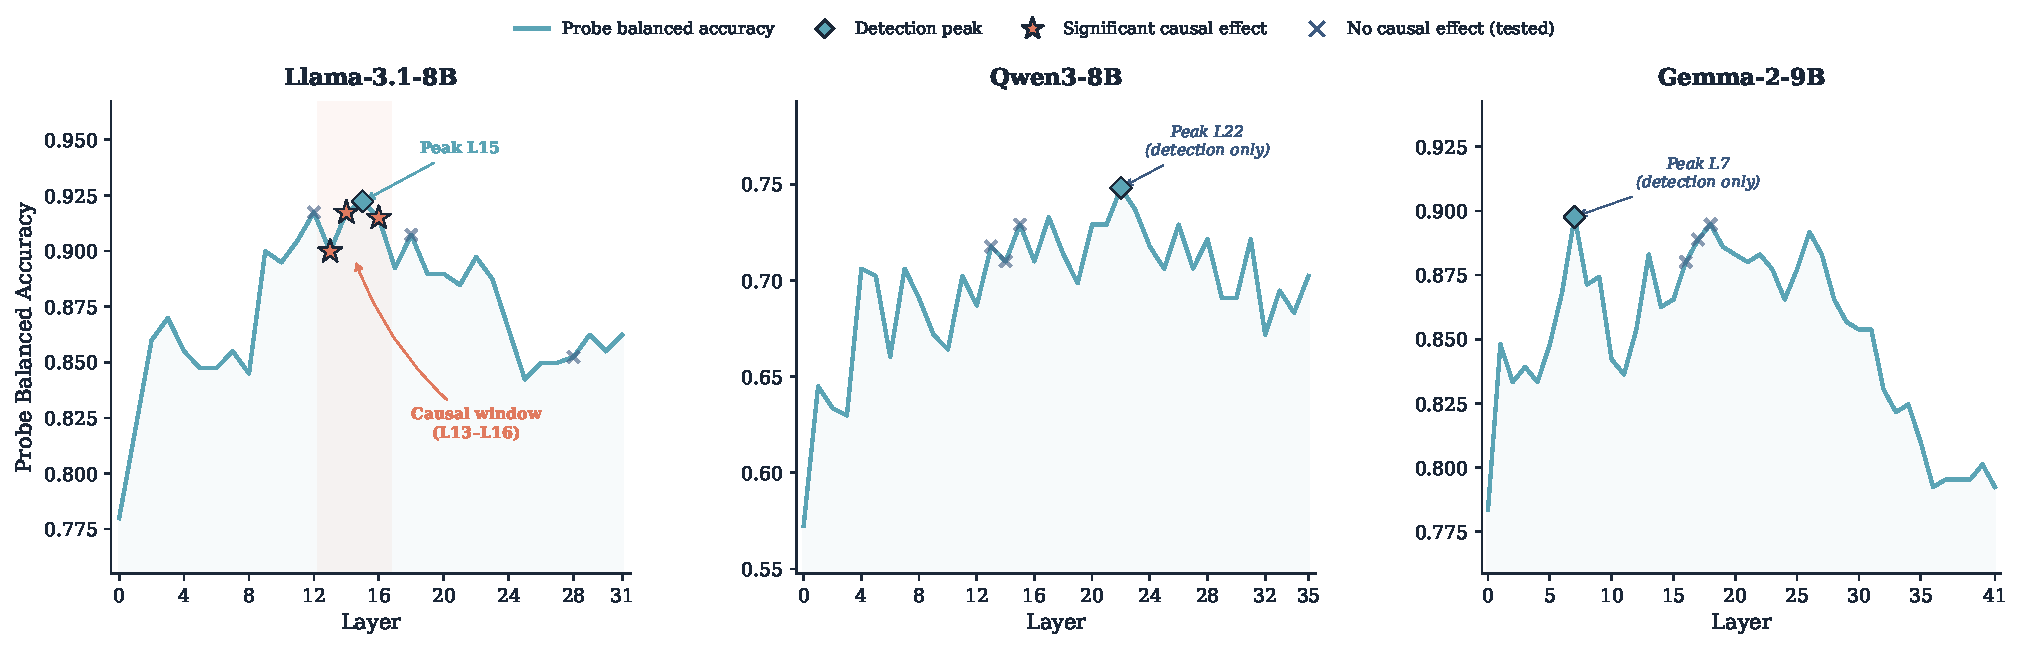
\includegraphics[width=\columnwidth]{fig6_dissociation.pdf}
\caption{Detection--decision dissociation across three architectures. For Llama, the linear probe peak (L15, 47\% depth), MLP probe peak (L18, 56\%), and causal steering node (L13, 41\%) cluster in mid-layers; upper layers (e.g., L28) retain detectable signal but lack causal influence. Qwen and Gemma achieve comparable probe accuracy but show no significant causal site under linear steering, illustrating that detectability does not imply causal relevance.}
\label{fig:dissociation}
\end{figure}

\section{AUROC Analysis}
\label{app:auroc}

Table~\ref{tab:auroc} reports AUROC for conflict probes on matched-condition replication data ($N = 131$--$201$), confirming strong continuous discriminative capacity across models.
Gemma's 0.93 EN$\to$EN AUROC (the highest among all models for this metric), paired with zero directional flips under steering, provides the strongest evidence that detection and causal influence are dissociable.

\begin{table}[!t]
\centering
\caption{AUROC and balanced accuracy for conflict probes (matched-condition data, best layer per model).}
\label{tab:auroc}
\small
\begin{tabular}{llcc}
\toprule
Model & Direction & AUROC & Bal.\ Acc (\%) \\
\midrule
Llama-3.1-8B & EN$\to$EN & 0.981 & 92.7 \\
\midrule
Gemma-2-9B-IT & EN$\to$EN & 0.931 & 88.1 \\
Gemma-2-9B-IT & ZH$\to$ZH & 0.900 & 85.7 \\
Gemma-2-9B-IT & EN$\to$ZH & 0.852 & 75.1 \\
Gemma-2-9B-IT & ZH$\to$EN & 0.921 & 77.8 \\
\midrule
Qwen3-8B & EN$\to$EN & 0.771 & 71.4 \\
\bottomrule
\end{tabular}
\end{table}

\section{Matched-Condition Steering Results}
\label{app:steering_config}

Table~\ref{tab:steering_config} reports steering results under matched conditions: all three architectures are tested at comparable relative depths (${\sim}$36--43\%) using the same probe training methodology and six $\alpha$ values in $[-20, +20]$.
Despite the highest probe accuracy among the three models (88--89\%), Gemma produces zero directional flips, ruling out probe quality as a confound for the Llama-specific positive result.
The full Llama causal gradient ($N = 201$) is in Appendix~\ref{app:boundary}.

\begin{table}[!t]
\centering
\caption{Matched-condition steering results. Probe: EN$\to$EN balanced accuracy at the target layer. Best $p$: minimum Fisher exact $p$-value across six tested $\alpha$ values. Bonf.: $\alpha$ values surviving Bonferroni correction out of 6. Flips: total directional transitions (p$\to$c $+$ c$\to$p).$^{\dagger}$}
\label{tab:steering_config}
\small
\begin{tabular}{lcrccc}
\toprule
Layer & Depth & Probe (\%) & Best $p$ & Bonf. & Flips \\
\midrule
\multicolumn{6}{l}{\textit{Llama-3.1-8B-Instruct ($N = 201$; 32 layers)}} \\
\textbf{L13} & \textbf{41\%} & \textbf{90.0} & $\mathbf{<0.001}$ & \textbf{2/6} & \textbf{9} \\
\midrule
\multicolumn{6}{l}{\textit{Qwen3-8B ($N = 131$; 36 layers)}} \\
L13 & 36\% & 71.8 & 0.168 & 0/6 & 0 \\
L14 & 39\% & 71.0 & 0.785 & 0/6 & 0 \\
L15 & 42\% & 72.9 & 0.617 & 0/6 & 0 \\
\midrule
\multicolumn{6}{l}{\textit{Gemma-2-9B-IT ($N = 171$; 42 layers)$^{\dagger}$}} \\
L16 & 38\% & 88.0 & 0.067 & 0/6 & 0 \\
L17 & 40\% & 88.9 & 0.448 & 0/6 & 0 \\
L18 & 43\% & 89.5 & 0.219 & 0/6 & 0 \\
\bottomrule
\end{tabular}
\begin{flushleft}
\footnotesize $^{\dagger}$ Gemma: after correcting a label assignment error.
\end{flushleft}
\end{table}

\section{Use of AI Assistance}
\label{app:ai-assistants}
We used Claude for coding, code drafting, debugging, and language polishing.

\end{document}
